\documentclass[10pt,a4paper]{article}
\usepackage[T1]{fontenc}
\usepackage[utf8]{inputenc}
\usepackage[polish]{babel}
\usepackage{lmodern,graphicx,booktabs,float,siunitx,enumitem,microtype,caption,amsmath}
\usepackage[margin=1.8cm]{geometry}
\sisetup{output-decimal-marker={,},group-digits=none}
\graphicspath{{images/}}
\setlength{\parindent}{0pt}
\setlength{\parskip}{4pt}
\setlength{\intextsep}{7pt}
\setlength{\textfloatsep}{8pt}
\setlist[enumerate]{leftmargin=*,itemsep=2pt,topsep=3pt}
\captionsetup{font=small}
\InputIfFileExists{author.tex}{}{\newcommand{\StudentNames}{Aleksander Łyskawa \quad Michał Klamecki}
\newcommand{\StudentIndices}{275462, 275486}
\newcommand{\LabGroup}{Grupa 2, 15:15--16:55}
}
\newcommand{\LinearMse}{\num{0.019045}}
\newcommand{\QuadraticMse}{\num{0.001459}}
\newcommand{\CubicMse}{\num{0.000734}}
\newcommand{\CubicNoisyMse}{\num{0.004171}}
\newcommand{\BestRidgeMse}{\num{0.000176}}
\newcommand{\BestLassoMse}{\num{0.000539}}
\newcommand{\RidgeGain}{\num{76.0}}
\newcommand{\LassoGain}{\num{26.6}}
\newcommand{\SurfaceGain}{\num{64.0}}
\newcommand{\SurfaceMaxCubic}{\num{1.056094}}

\begin{document}
\noindent\begin{minipage}{\linewidth}\centering
{\Large MNK i regresja wielomianowa}\\[3pt]
Ćwiczenie 2 -- Analiza danych eksperymentalnych\\[5pt]
{\small\StudentNames}\\[2pt]
{\small Prowadzący: \Instructor\quad |\quad\LabGroup\quad |\quad 3 listopada 2026}
\end{minipage}
\vspace{-3pt}

\section*{Zadanie 1. Aproksymacja funkcji jednej zmiennej}
Wygenerowaliśmy $N=25$ argumentów $x_i=4(i-1)/(N-1)$ dla $i=1,\ldots,N$
oraz wartości $y_{0,i}=\log_2(x_i+1)$ i $y_i=y_{0,i}+\varepsilon_i$.
Niezależny szum $\varepsilon_i$ ma rozkład normalny o średniej 0 i odchyleniu
standardowym \num{0.1}; ziarno generatora to 2026. Do zaszumionych $y_i$ dopasowaliśmy MNK wielomiany
$p_d(x)=\sum_{j=0}^{d}a_jx^j$ stopnia $d=1,2,3$.
$\mathrm{MSE}_0$ i $R_0^2$ porównują model z wartościami bez szumu w tych samych
25 punktach; $R_y^2$ opisuje dopasowanie do danych zaszumionych.

\begin{table}[H]\centering\small
\setlength{\tabcolsep}{4pt}
\begin{tabular}{lrrrrrrr}
\toprule
Stopień & $a_0$ & $a_1$ & $a_2$ & $a_3$ & $R_y^2$ & $R_0^2$ & $\mathrm{MSE}_0$ \\
\midrule
1 & \num{0.355668} & \num{0.542735} & -- & -- & \num{0.941099} & \num{0.956780} & \num{0.019045} \\
2 & \num{0.082301} & \num{0.970613} & \num{-0.106970} & -- & \num{0.983140} & \num{0.996690} & \num{0.001459} \\
3 & \num{-0.039868} & \num{1.379371} & \num{-0.367724} & \num{0.043459} & \num{0.990774} & \num{0.998334} & \num{0.000734} \\
\bottomrule
\end{tabular}

\caption{Współczynniki w bazie $1,x,x^2,x^3$ oraz jakość aproksymacji.}
\end{table}
\begin{figure}[H]\centering
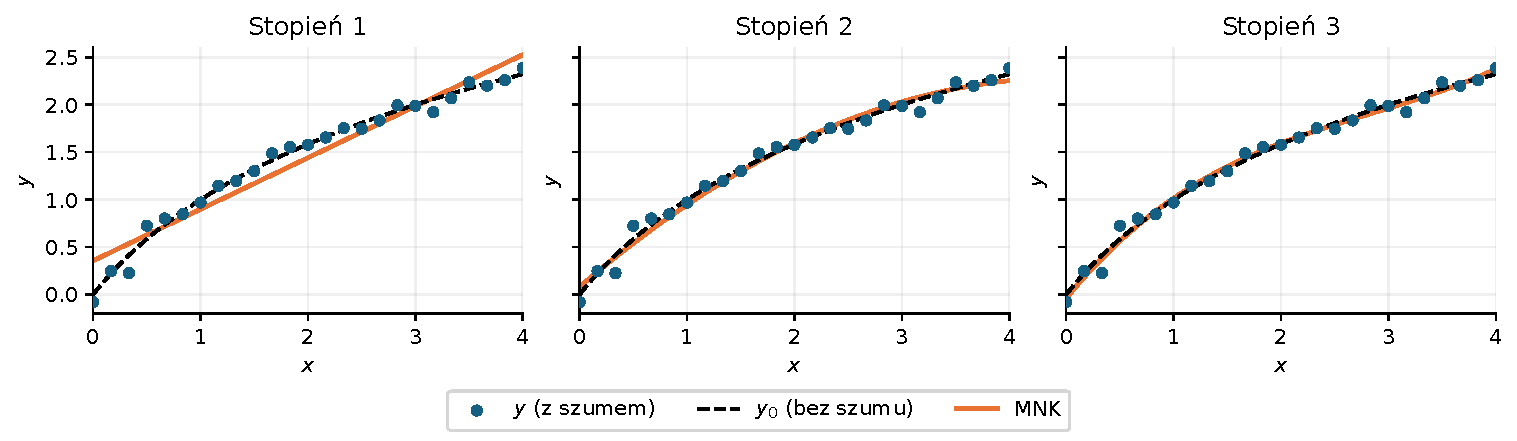
\includegraphics[width=\linewidth]{task1_polynomials.pdf}
\caption{Wspólne dane i zakresy osi dla trzech stopni wielomianu.}
\end{figure}

\textbf{Układ nadokreślony dla stopnia 3.}
Rozwiązaliśmy $\mathbf A\mathbf a\approx\mathbf y$, czyli minimalizowaliśmy
$\|\mathbf e\|_2^2$, gdzie $\mathbf e=\mathbf y-\mathbf A\mathbf a$ jest wektorem reszt:
\[
\mathbf A=\begin{bmatrix}
1&x_1&x_1^2&x_1^3\\
1&x_2&x_2^2&x_2^3\\
\vdots&\vdots&\vdots&\vdots\\
1&x_{25}&x_{25}^2&x_{25}^3
\end{bmatrix}_{25\times4},\qquad
\mathbf a=\begin{bmatrix}a_0\\a_1\\a_2\\a_3\end{bmatrix}_{4\times1},\qquad
\mathbf y=\begin{bmatrix}y_1\\y_2\\\vdots\\y_{25}\end{bmatrix}_{25\times1}.
\]
Indeks $i$ numeruje obserwacje, $j$ -- potęgi argumentu; $a_j$ to szukane
współczynniki, a $\mathbf e$ ma rozmiar $25\times1$.

\textbf{Obliczenie MNK.}
Użyliśmy \texttt{numpy.linalg.lstsq} z \texttt{rcond=None}, opartej na procedurze
LAPACK \texttt{gelsd}. Algorytm redukuje macierz przekształceniami Householdera
do postaci bidiagonalnej, rozwiązuje problem metodą dziel i zwyciężaj
i przekształca wynik z powrotem.
Dla pełnego rzędu kolumnowego wynik można zapisać jako
$\mathbf A=\mathbf U\boldsymbol\Sigma\mathbf V^T$,
$\widehat{\mathbf a}=\mathbf V\boldsymbol\Sigma^{-1}\mathbf U^T\mathbf y$.
Macierze $\mathbf U$ ($25\times4$) i $\mathbf V$ ($4\times4$) mają ortonormalne kolumny;
$\boldsymbol\Sigma$ ($4\times4$) jest diagonalna i zawiera dodatnie wartości osobliwe.
Symbol $T$ oznacza transpozycję, a $\widehat{\mathbf a}$ -- wyznaczone współczynniki.
Funkcja odrzuca numerycznie zaniedbywalne wartości osobliwe; tutaj rząd wyniósł 4.
Nie tworzyliśmy macierzy $\mathbf A^T\mathbf A$.

\textbf{Wnioski}
\begin{enumerate}
\item Prosta słabo odtwarza krzywiznę logarytmu: $\mathrm{MSE}_0=\LinearMse$.
\item Wielomian kwadratowy obniża ten błąd do \QuadraticMse; największa poprawa wynika z uwzględnienia krzywizny.
\item Wśród modeli MNK najlepszy jest wielomian sześcienny: $\mathrm{MSE}_0=\CubicMse$.
\item Dla stopnia 3 błąd względem $y$ wynosi \CubicNoisyMse, czyli jest większy od błędu względem $y_0$.
\item Cztery współczynniki przy 25 obserwacjach nie pozwalają interpolować wszystkich zaszumionych punktów.
\end{enumerate}

\clearpage
\section*{Zadanie 2. Ridge i LASSO}
Zachowaliśmy dokładnie te same 25 obserwacji co w zadaniu 1.
Przed regularyzacją wystandaryzowaliśmy każdą kolumnę $x^j$ osobno:
$Z_{ij}=(x_i^j-m_j)/s_j$, gdzie $m_j$ to średnia, a $s_j$ -- odchylenie
standardowe z dzielnikiem $N=25$. Macierz $\mathbf Z$ ma rozmiar $25\times d$.
Wyraz wolny $b$ pozostawiliśmy bez kary. Minimalizowane kryteria miały postać:
\[
\begin{aligned}
\text{Ridge:}\quad&\|\mathbf y-b\mathbf 1-\mathbf Z\mathbf w\|_2^2+\alpha\|\mathbf w\|_2^2,\\
\text{LASSO:}\quad&\frac{1}{2N}\|\mathbf y-b\mathbf 1-\mathbf Z\mathbf w\|_2^2+\alpha\|\mathbf w\|_1.
\end{aligned}
\]
$\mathbf w$ zawiera $d$ wag przeskalowanych cech, $\mathbf 1$ to wektor 25 jedynek,
a $\alpha>0$ określa siłę kary. Norma $\|\mathbf w\|_1$ jest sumą modułów wag,
a $\|\mathbf w\|_2^2$ -- sumą ich kwadratów.
Ze względu na czynnik $1/(2N)$ tych samych wartości $\alpha$ nie porównujemy
bezpośrednio między metodami. Ridge obliczyliśmy przez SVD, a LASSO przez
cykliczne aktualizowanie pojedynczych wag (spadek współrzędnych).
W tabelach podajemy współczynniki w oryginalnej bazie:
$a_j=w_j/s_j$ dla $j\geq1$ i $a_0=b-\sum_{j=1}^{d}w_jm_j/s_j$.
Wiersze MNK są punktem odniesienia; wszystkie błędy dotyczą danych bez szumu.

\begin{table}[H]\centering\small
\begin{tabular}{lrrrrr}
\toprule
Metoda & $\alpha$ & $a_0$ & $a_1$ & $a_2$ & $\mathrm{MSE}_0$ \\
\midrule
MNK & -- & \num{0.082301} & \num{0.970613} & \num{-0.106970} & \num{0.001459} \\
Ridge & \num{0.0100} & \num{0.088093} & \num{0.962367} & \num{-0.105004} & \num{0.001436} \\
Ridge & \num{0.1000} & \num{0.134918} & \num{0.895891} & \num{-0.089185} & \num{0.001741} \\
Ridge & \num{1.0000} & \num{0.361180} & \num{0.583862} & \num{-0.016120} & \num{0.014584} \\
Ridge & \num{10.0000} & \num{0.676467} & \num{0.274746} & \num{0.039523} & \num{0.051827} \\
LASSO & \num{0.0001} & \num{0.083973} & \num{0.968174} & \num{-0.106381} & \num{0.001451} \\
LASSO & \num{0.0010} & \num{0.099018} & \num{0.946220} & \num{-0.101079} & \num{0.001433} \\
LASSO & \num{0.0100} & \num{0.249474} & \num{0.726678} & \num{-0.048066} & \num{0.006481} \\
LASSO & \num{0.1000} & \num{0.522078} & \num{0.459530} & \num{0.000000} & \num{0.028456} \\
\bottomrule
\end{tabular}

\caption{Wielomiany stopnia 2: $p_2(x)=a_0+a_1x+a_2x^2$.}
\end{table}
\begin{table}[H]\centering\small
\begin{tabular}{lrrrrrr}
\toprule
Metoda & $\alpha$ & $a_0$ & $a_1$ & $a_2$ & $a_3$ & $\mathrm{MSE}_0$ \\
\midrule
MNK & -- & \num{-0.039868} & \num{1.379371} & \num{-0.367724} & \num{0.043459} & \num{0.000734} \\
Ridge & \num{0.0100} & \num{0.011548} & \num{1.225355} & \num{-0.274978} & \num{0.028559} & \num{0.000176} \\
Ridge & \num{0.1000} & \num{0.140095} & \num{0.871693} & \num{-0.071530} & \num{-0.003174} & \num{0.002003} \\
Ridge & \num{1.0000} & \num{0.335360} & \num{0.581158} & \num{0.015843} & \num{-0.008568} & \num{0.010553} \\
Ridge & \num{10.0000} & \num{0.691213} & \num{0.254413} & \num{0.032007} & \num{0.004011} & \num{0.057330} \\
LASSO & \num{0.0001} & \num{-0.028906} & \num{1.345849} & \num{-0.347307} & \num{0.040154} & \num{0.000539} \\
LASSO & \num{0.0010} & \num{0.069748} & \num{1.044152} & \num{-0.163552} & \num{0.010412} & \num{0.000631} \\
LASSO & \num{0.0100} & \num{0.246502} & \num{0.681040} & \num{0.000000} & \num{-0.010047} & \num{0.005650} \\
LASSO & \num{0.1000} & \num{0.522078} & \num{0.459530} & \num{0.000000} & \num{0.000000} & \num{0.028456} \\
\bottomrule
\end{tabular}

\caption{Wielomiany stopnia 3: $p_3(x)=a_0+a_1x+a_2x^2+a_3x^3$.}
\end{table}
\begin{figure}[H]\centering
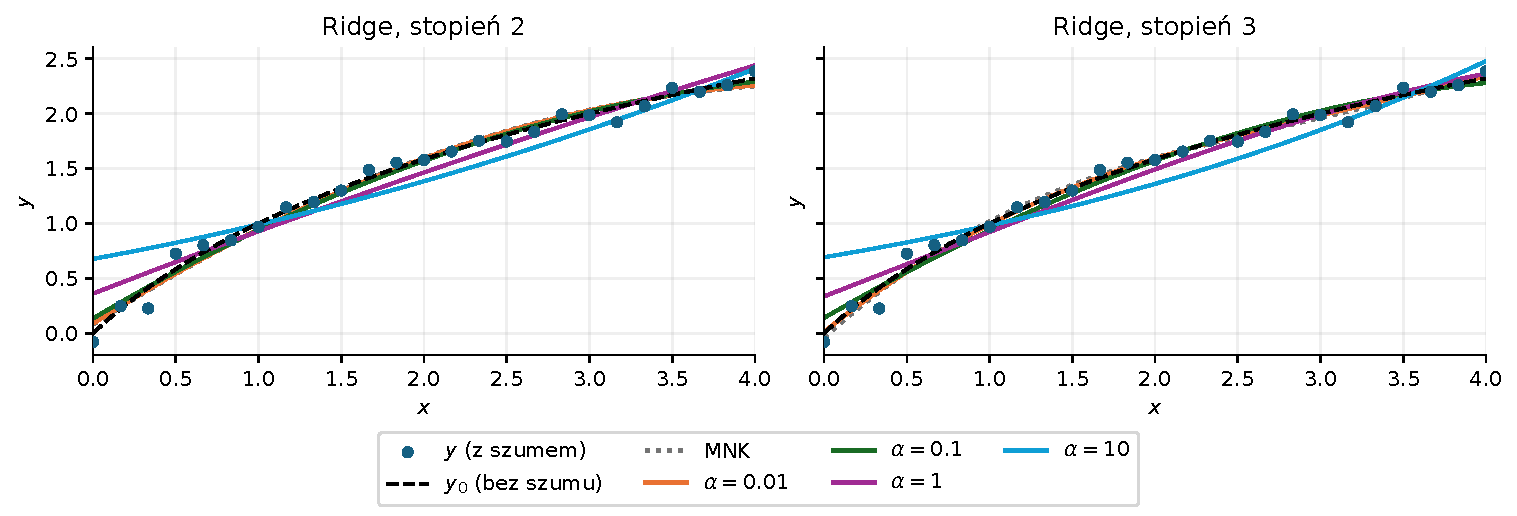
\includegraphics[width=\linewidth]{task2_ridge.pdf}
\caption{Ridge przy rosnącej regularyzacji. Krzywe dla słabych kar częściowo się pokrywają.}
\end{figure}

\clearpage
\section*{Zadanie 2. Porównanie wyników (cd.)}
\begin{figure}[H]\centering
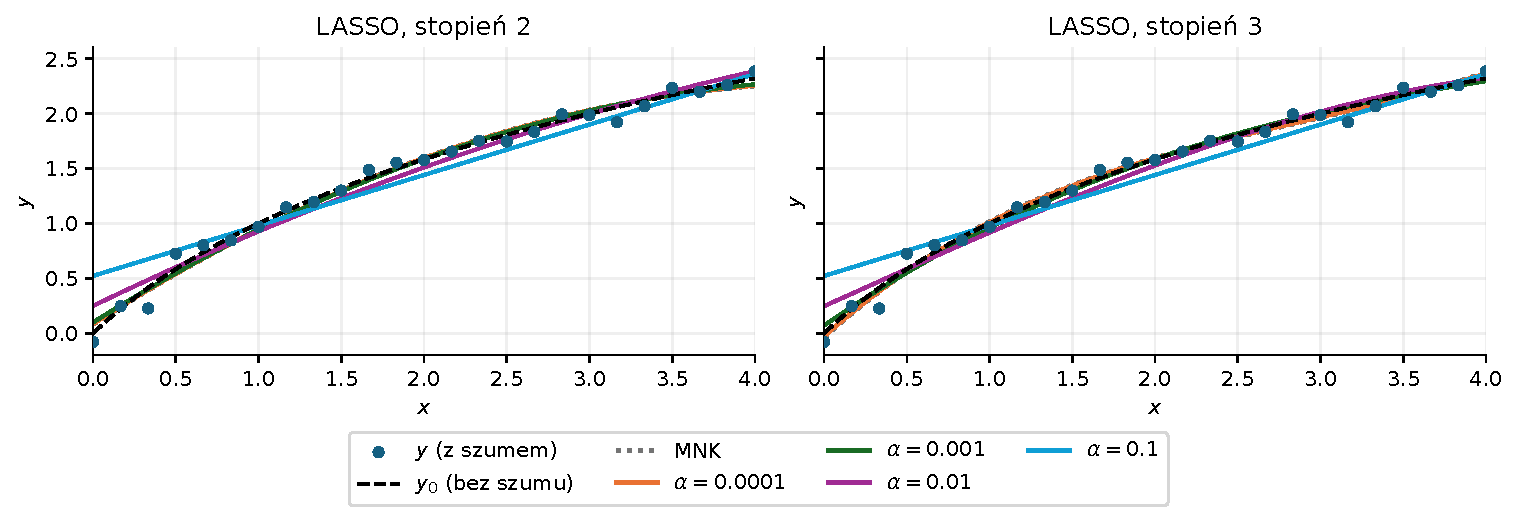
\includegraphics[width=\linewidth]{task2_lasso.pdf}
\caption{LASSO przy rosnącej regularyzacji, z tymi samymi danymi co dla Ridge.}
\end{figure}
\textbf{Wnioski}
\begin{enumerate}
\item Najmniejszy błąd wśród zbadanych ustawień daje Ridge stopnia 3 z $\alpha=\num{0.01}$:
      $\mathrm{MSE}_0=\BestRidgeMse$, o \RidgeGain\% mniej niż MNK tego samego stopnia.
\item Najlepszy wariant LASSO to stopień 3 z $\alpha=\num{0.0001}$:
      $\mathrm{MSE}_0=\BestLassoMse$, poprawa o \LassoGain\% względem MNK.
\item Dla stopnia 2 niewielka regularyzacja także pomaga, lecz poprawa jest mała.
      Duża kara pogarsza wynik w obu metodach i dla obu stopni.
\item Ridge nie zeruje wag w badanych wariantach. Współczynniki w oryginalnej bazie
      nie muszą maleć pojedynczo: karę nakładaliśmy na wagi cech po standaryzacji.
\item LASSO z $\alpha=\num{0.01}$ usuwa składnik $x^2$ modelu sześciennego,
      ale zachowuje $x^3$. Przy $\alpha=\num{0.1}$ oba modele LASSO redukują się do tej samej prostej.
\item Silna regularyzacja spłaszcza przebieg i utrudnia odtworzenie krzywizny funkcji.
      Wyraźnie widać to przy końcach przedziału.
\item Najlepsze $\alpha$ wskazaliśmy na podstawie znanej funkcji bez szumu.
      Jest to porównanie tej realizacji danych i wybranych kar, a nie wynik walidacji na niezależnych pomiarach.
\end{enumerate}

\section*{Zadanie 3. Funkcja dwóch zmiennych -- układ MNK}
Wylosowaliśmy niezależnie 200 par $(x_i,y_i)$ z rozkładu jednostajnego
na $[0,4)\times[0,4)$, z ziarnem 2027. Obliczyliśmy bez szumu
$z_i=f(x_i,y_i)=\sin\!\bigl(\ln(x_i+2)\sqrt{2y_i}\bigr)$.
Dopasowaliśmy pełne wielomiany całkowitego stopnia 2 i 3, łącznie z wyrazami mieszanymi.

Rozwiązaliśmy $\mathbf A_d\mathbf c_d\approx\mathbf z$ metodą MNK:
\[
\mathbf A_2=\begin{bmatrix}
1&x_1&y_1&x_1^2&x_1y_1&y_1^2\\
\vdots&\vdots&\vdots&\vdots&\vdots&\vdots\\
1&x_{200}&y_{200}&x_{200}^2&x_{200}y_{200}&y_{200}^2
\end{bmatrix}_{200\times6},
\]
\[
\mathbf A_3=\left[\ \mathbf A_2\ \middle|\ \begin{matrix}
x_1^3&x_1^2y_1&x_1y_1^2&y_1^3\\
\vdots&\vdots&\vdots&\vdots\\
x_{200}^3&x_{200}^2y_{200}&x_{200}y_{200}^2&y_{200}^3
\end{matrix}\ \right]_{200\times10}.
\]
Indeks $i=1,\ldots,200$ oznacza obserwację, a $d$ -- stopień wielomianu.
Wektor $\mathbf z=[z_1,\ldots,z_{200}]^T$ ma rozmiar $200\times1$.
$\mathbf c_2=[c_0,c_x,c_y,c_{x^2},c_{xy},c_{y^2}]^T$ ma rozmiar $6\times1$;
$\mathbf c_3$ ma ten sam porządek wyrazów, z dodatkowymi wagami
$[c_{x^3},c_{x^2y},c_{xy^2},c_{y^3}]^T$, i rozmiar $10\times1$.
Każdy $c$ jest współczynnikiem przy wskazanym jednomianie; jego wartość wyznaczamy osobno dla każdego stopnia.
Wektor reszt $\mathbf z-\mathbf A_d\mathbf c_d$ ma rozmiar $200\times1$.
Użyliśmy tego samego algorytmu SVD co w zadaniu 1; rzędy macierzy wyniosły odpowiednio 6 i 10.

\clearpage
\section*{Zadanie 3. Wyniki aproksymacji}
Współczynniki w tabeli~\ref{tab:surface-coefficients} mnożymy przez wyrazy z pierwszej kolumny i sumujemy.
Ocenę poza punktami uczenia wykonaliśmy na regularnej siatce $40\times40$
obejmującej cały kwadrat $[0,4]^2$, wraz z brzegami.
Wszystkie błędy obliczyliśmy z pełnej precyzji współczynników.

\begin{minipage}[t]{0.39\linewidth}\vspace{0pt}\centering\small
\begin{tabular}{lrr}
\toprule
Wyraz & Stopień 2 & Stopień 3 \\
\midrule
$1$ & \num{0.730258} & \num{-0.204174} \\
$x$ & \num{0.036078} & \num{0.902749} \\
$y$ & \num{0.307682} & \num{1.706135} \\
$x^2$ & \num{0.020220} & \num{-0.255641} \\
$xy$ & \num{-0.216718} & \num{-0.689203} \\
$y^2$ & \num{-0.067059} & \num{-0.679498} \\
$x^3$ & -- & \num{0.027180} \\
$x^2y$ & -- & \num{0.056439} \\
$xy^2$ & -- & \num{0.065496} \\
$y^3$ & -- & \num{0.082091} \\
\bottomrule
\end{tabular}

\captionof{table}{Współczynniki obu powierzchni.}\label{tab:surface-coefficients}
\end{minipage}\hfill
\begin{minipage}[t]{0.57\linewidth}\vspace{0pt}\centering\small
\setlength{\tabcolsep}{4pt}
\begin{tabular}{lrrr}
\toprule
Stopień & $\mathrm{MSE}_{\mathrm{ucz}}$ & $\mathrm{MSE}_{\mathrm{siatka}}$ & $\max|f-p|$ \\
\midrule
2 & \num{0.024589} & \num{0.053726} & \num{1.198096} \\
3 & \num{0.005419} & \num{0.019339} & \num{1.056094} \\
\bottomrule
\end{tabular}

\captionof{table}{Błąd na 200 punktach uczenia i 1600 punktach siatki. Maksimum dotyczy siatki.}
\raggedright\normalsize
\vspace{4pt}
$\mathrm{MSE}_{\mathrm{ucz}}$ jest średnim kwadratem reszt w punktach dopasowania.
$\mathrm{MSE}_{\mathrm{siatka}}$ porównuje $p_d$ z funkcją $f$ na siatce.
Na wykresach po prawej pokazaliśmy błąd ze znakiem $f-p_d$.
Oba wykresy aproksymacji mają wspólny zakres osi pionowej;
oba wykresy błędu także mają wspólną, symetryczną skalę.
\end{minipage}

\begin{figure}[H]\centering
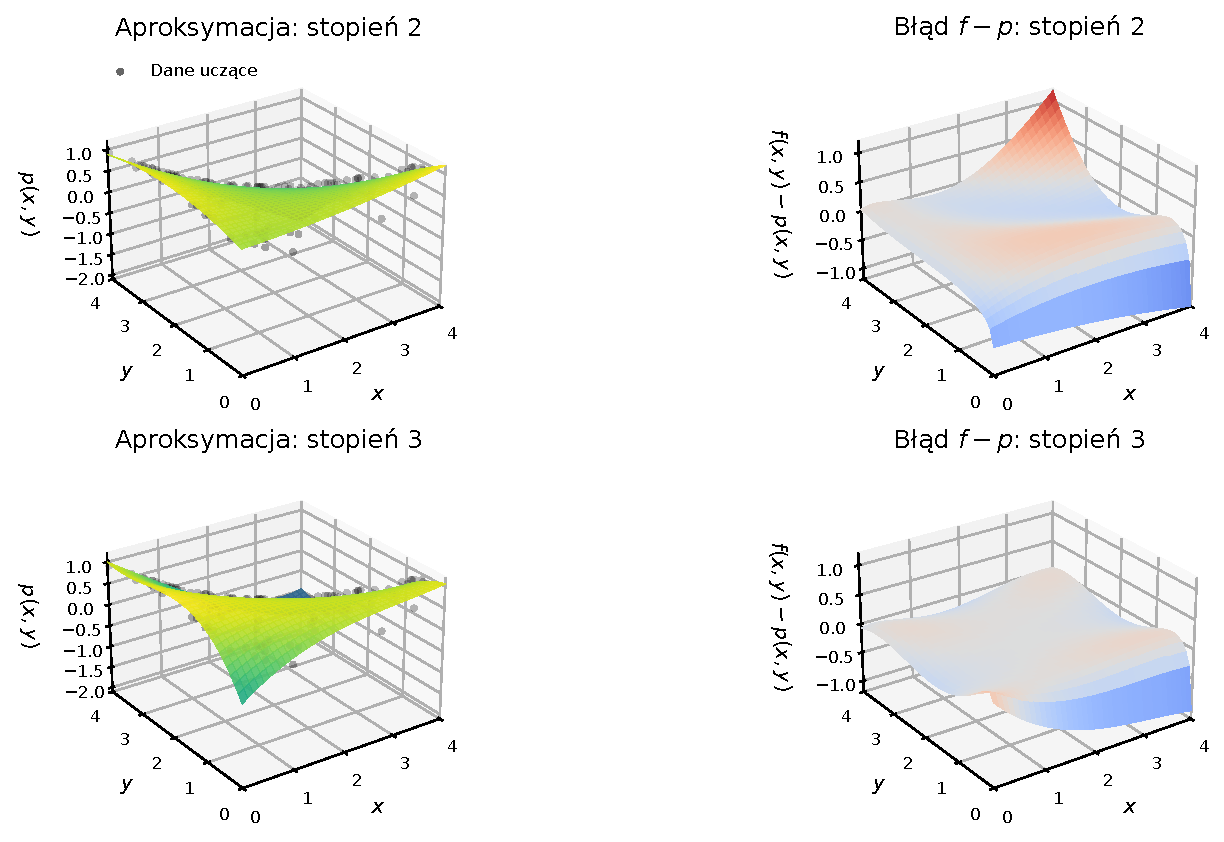
\includegraphics[width=\linewidth]{task3_surfaces.pdf}
\caption{Powierzchnie MNK (lewa kolumna) i ich błędy (prawa kolumna). Czarne punkty oznaczają dane uczące.}
\end{figure}
\textbf{Wnioski}
\begin{enumerate}
\item Stopień 3 lepiej odtwarza krzywiznę: zmniejsza błąd siatki o \SurfaceGain\% względem stopnia 2.
\item Dla obu modeli błąd na siatce jest większy niż w punktach uczenia.
\item Największy błąd siatki występuje w $(4,0)$; dla stopnia 3 nadal wynosi \SurfaceMaxCubic.
\item Modele nie zachowują warunku $f(x,0)=0$. Brzeg $y=0$ nie zawiera punktów uczenia;
      dopasowanie nie narzuca tam zerowej wartości modelu.
\item Wykres błędu pokazuje strukturę niewyjaśnioną przez wielomian, mimo braku szumu w danych.
\end{enumerate}
\end{document}
